\documentclass{article}

\usepackage{fancyhdr}
\usepackage{extramarks}
\usepackage{amsmath}
\usepackage{amsthm}
\usepackage{amsfonts}
\usepackage{tikz}
\usepackage[plain]{algorithm}
\usepackage{algpseudocode}
\usepackage{enumerate}
\usepackage{braket}
\usepackage{color}
\usepackage{fontspec}
\usepackage{subfig}
\usepackage{booktabs}
\usepackage{multirow}

\usetikzlibrary{automata,positioning}

%
% Basic Document Settings
%

\topmargin=-0.45in
\evensidemargin=0in
\oddsidemargin=0in
\textwidth=6.5in
\textheight=9.0in
\headsep=0.25in

\linespread{1.1}

\pagestyle{fancy}
\lhead{\hmwkAuthorName}
\rhead{\hmwkClassNo: \hmwkTitle}
\cfoot{\thepage}

\renewcommand\headrulewidth{0.4pt}
\renewcommand\footrulewidth{0.4pt}

\setlength\parindent{0pt}

\newcommand{\hmwkTitle}{Homework Project\ \#4}
\newcommand{\hmwkDueDate}{April 14, 2023}
\newcommand{\hmwkClass}{Monte Carlo and Molecular Dynamics Simulation in Statistical Physics \& Materials Science}
\newcommand{\hmwkClassNo}{MSE504}
\newcommand{\hmwkClassInstructor}{Professor R. Car}
\newcommand{\hmwkAuthorName}{\textbf{Yihang Peng}}

%
% Title Page
%

\title{
    \vspace{2in}
    \textmd{\textbf{\hmwkClassNo\ -\ \hmwkClass:\ \hmwkTitle}}\\
    \normalsize\vspace{0.1in}\small{Due\ on\ \hmwkDueDate\ at 11:59 p.m.}\\
    \vspace{0.1in}\large{\textit{\hmwkClassInstructor}}
    \vspace{3in}
}

\author{\hmwkAuthorName}
\date{}

\newcommand{\pderiv}[2]{\frac{\partial #1}{\partial #2}}
\newcommand{\bpp}[3]{\left(\frac{\partial #1}{\partial #2}\right)_{#3}}
\newcommand{\dx}{\mathrm{d}x}
\newcommand{\E}{\mathrm{E}}
\newcommand{\Var}{\mathrm{Var}}
\newcommand{\Cov}{\mathrm{Cov}}
\newcommand{\Bias}{\mathrm{Bias}}
\newcommand{\diff}[1]{\mathrm{d} #1}
\newcommand{\e}[1]{\times 10^{#1}}
\newcommand{\Exp}[1]{\mathrm{e}^{#1}}
\newcommand{\mathpth}{\text{\pth}}
\newcommand{\inv}{^{-1}}
\newcommand{\ang}[1]{{\langle #1 \rangle}}

\setlength{\parskip}{1em}

\begin{document}

\maketitle

\pagebreak

The Hamiltonian of a classical harmonic oscillator in 1 d is
\begin{equation}
    \mathcal{H} = \frac{p^2}{2m} + \frac{1}{2} m \omega^2 x^2
\end{equation}
Since $m = \omega = 1$, we have
\begin{equation}
    \mathcal{H} = \frac{1}{2} p^2 + \frac{1}{2} x^2
\end{equation}
Therefore, the force acting on the oscillator is given by
\begin{equation}
    F = - \pderiv{\varPhi}{x} = - \pderiv{\left(\frac{1}{2}x^2\right)}{x} = -x
\end{equation}

\section{Coupling to a single Nose-Hoover thermostat}
Considering a single Nose-Hoover thermostat, the equations of motion of the 1D single particle coupled system is given by
\begin{equation}
    \begin{aligned}
        \dot{x} & = \frac{p}{m} \\
        \dot{p} & = F-\zeta p \\
        \dot{\zeta} & =\frac{1}{Q}\left(\frac{p^2}{m}-k_B T\right)
    \end{aligned}
\end{equation}
where $\zeta$ is a dynamic friction coefficient, and $Q$ is a constant that plays the role of friction ``mass''. Since $m = \omega = 1$, we obtain
\begin{equation}
    \begin{aligned}
        \dot{x} & = p \\
        \dot{p} & = F-\zeta p \\
        \dot{\zeta} & =\frac{1}{Q}\left(p^2 - 1\right)
    \end{aligned}
\end{equation}
Here take $k_B T = 1$ to simplify the calculation. The boundary condition for the differential equations is set to $x_0 = 1,\ p_0 = 0$. The time step of this calculation is 0.0001, and the total number of steps is 1,000,000. In order to find the appropriate mass, I solve the equations of motion with different $Q$ increasing from 0.05 to 0.6, in increments of 0.05. The corresponding trajectories in the $p$-$x$ phase plane are plotted as shown in Fig. 1. For $Q \geq 0.2$, the trajectories of the harmonic oscillator are in a circle shape, because this is an integrable system and the motion of it is confined to an invariant torus in phase space. However, if $Q$ is lower than or equal to 0.15, the torus profile no longer exists. 

According to the Kolmogorov-Arnold-Moser (KAM) theorem, a nonlinear perturbation applied to a finite integrable system will destroy the invariant torus (resulting in ergodic behavior) only when the perturbation exceeds some finite threshold. As the friction ``mass'', $Q$ plays the role of the perturbation on the system, and decreasing $Q$ results in the increase of perturbation to the momentum as shown in Eq. 4. The perturbation only reaches the threshold when Q is reduced to 0.15 or below, at which the torus-shaped trajectory is destroied. It's worth noting that as $Q$ approaches this critical value near 0.15, the trajectory exhibits extremely irregular features, and then a unique double diamond shape emerges after $Q$ is reduced to 0.1. Therefore, my results is consistent with KAM theorem and I find that the threshold of this harmonic oscillator system is between 0.15 and 0.20.

\begin{figure}[p]
    \centering
    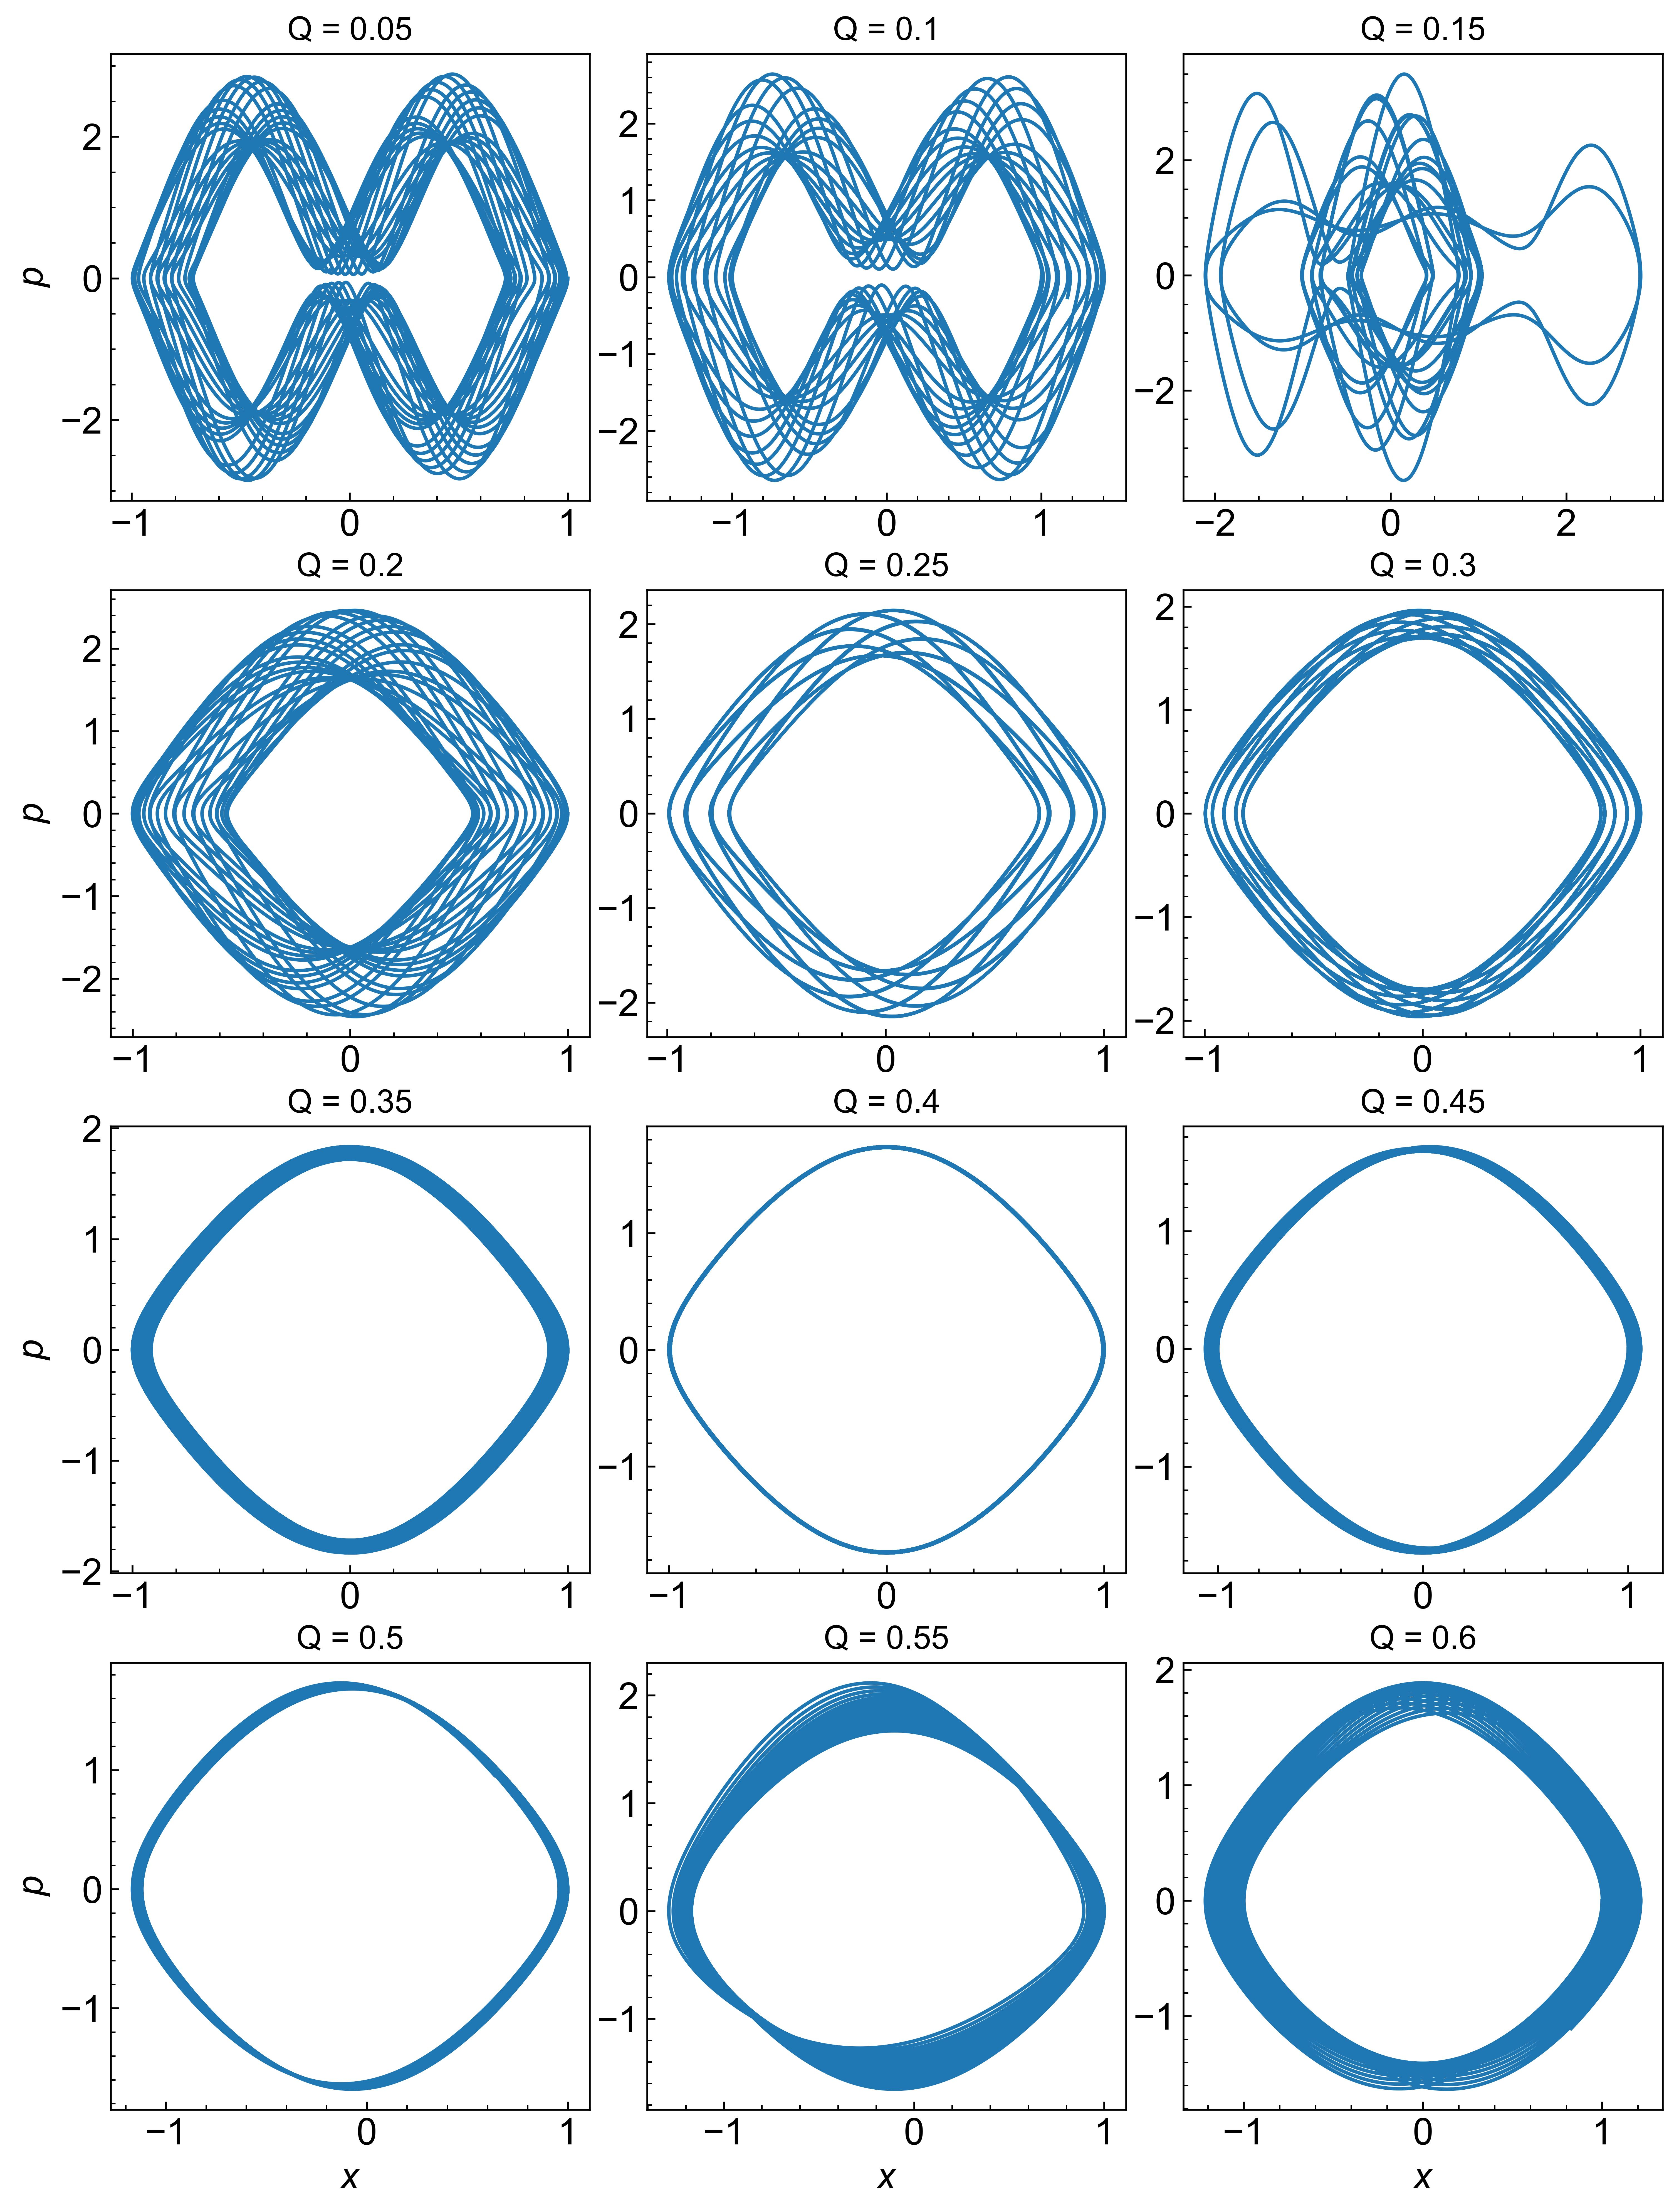
\includegraphics[width=\textwidth]{fig1.jpg}
    \caption{The trajectories in the $p$-$x$ phase plane of a harmonic oscillator coupled to a single Nose-Hoover thermostat with different $Q$.}
\end{figure}

\section{Coupling to a Nose-Hoover chain}
Considering a Nose-Hoover chain of $M$ Nose-Hoover thermostat, the equations of motion of the 1D single particle coupled system is
\begin{equation}
    \begin{array}{ll}
        \dot{x}=\frac{p}{m} & \\
        \dot{p}=F-\frac{p_{\eta_1}}{Q_1} p & \\
        \dot{\eta}_k=\frac{p_{\eta_k}}{Q_k} & (k=1, \ldots, M-1) \\
        \dot{p}_{\eta_k}=G_k-\frac{p_{\eta_{k+1}}}{Q_{k+1}} p_{\eta_k} & \\
        \dot{p}_{\eta_M}=G_M
    \end{array}
\end{equation}
Here $G_1=\frac{p^2}{m}-k_B T$ and $G_k=\frac{\dot{p}_{\eta_{k-1}}^2}{Q_{k-1}}-k_B T$ $(k=2, \cdots, M)$. I still take $m = \omega = 1$, $F = -x$, and $k_B T =1$. After tuning the parameters, I set $k_B T = 1$, $M = 6$, $Q_1 = Q_2 = \cdots = Q_6 = 0.4$. The boundary condition is set to $x_0 = 1,\ p_0 = 0$. The time step of this calculation is 0.001, and the total number of steps is 10,000,000. The corresponding trajectories in the $p$-$x$ phase plane are plotted as shown in Fig. 2.

\begin{figure}[h!]
    \centering
    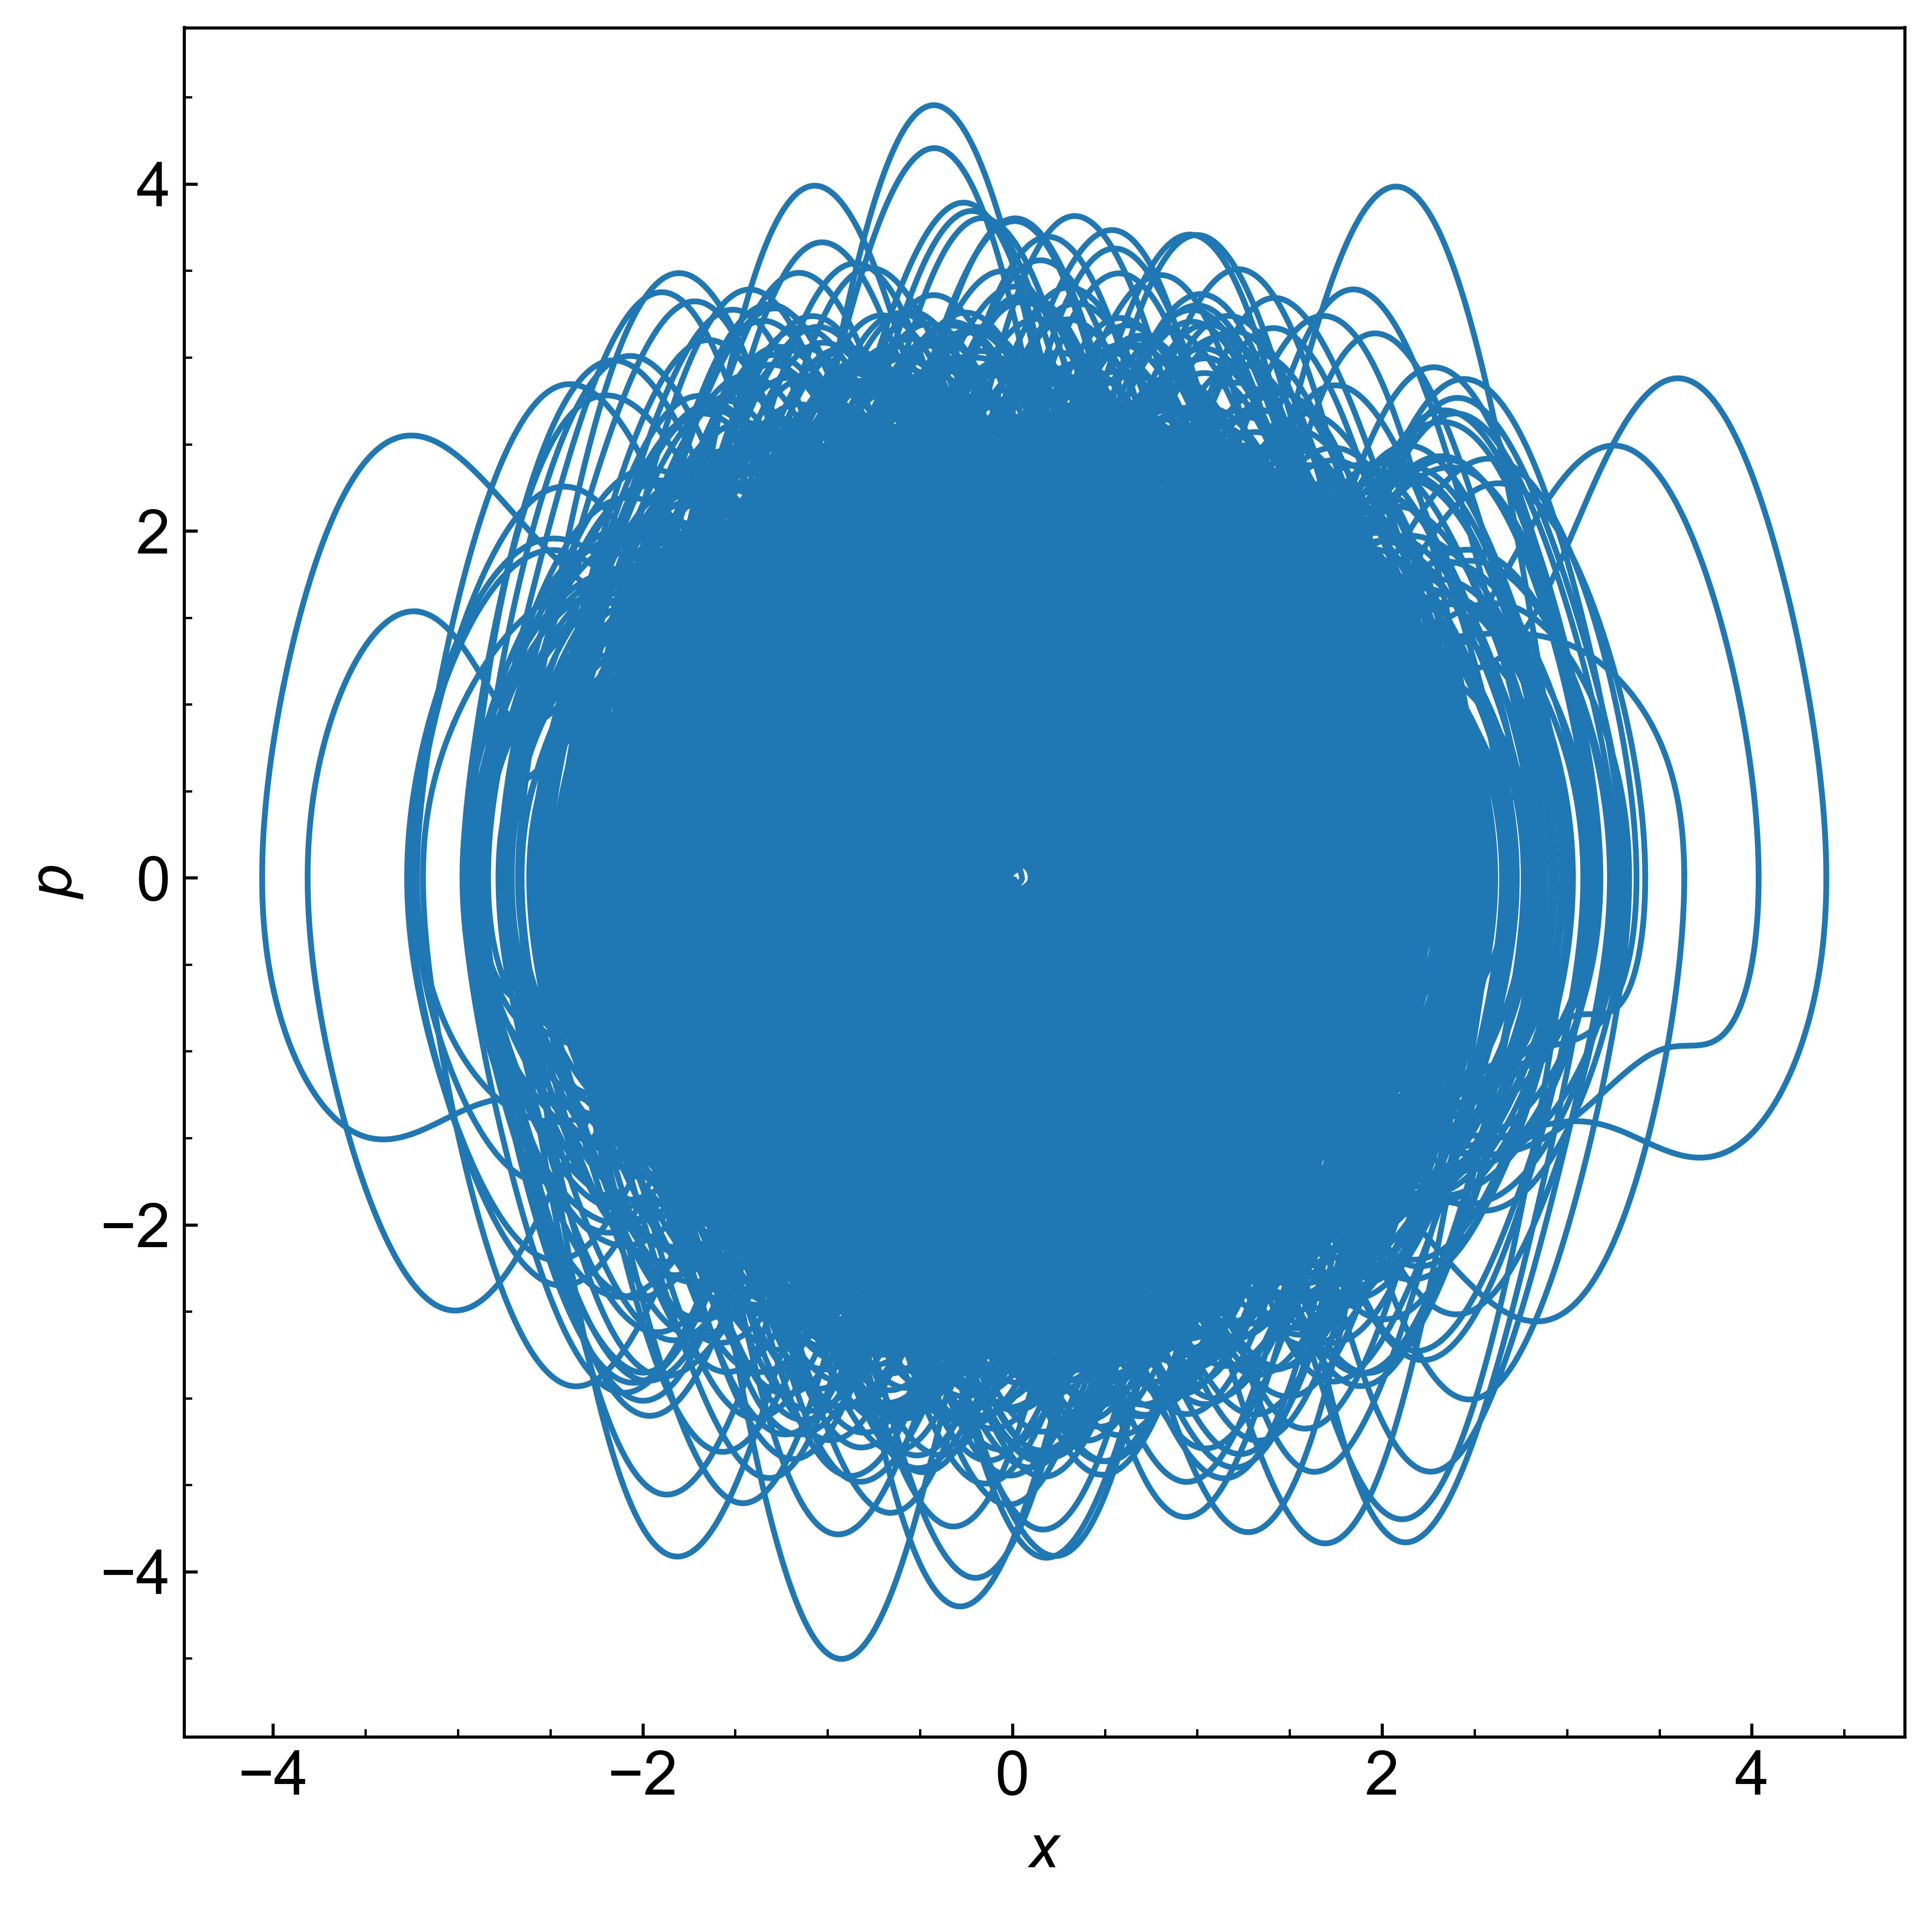
\includegraphics[width=0.65\textwidth]{NHchain.jpg}
    \caption{The trajectories in the $p$-$x$ phase plane of a harmonic oscillator coupled to a Nose-Hoover chain of 6 Nose-Hoover thermostat with $Q = 0.4$.}
\end{figure}

Considering a canonical ensemble, the distribution of position and momentum of particles follow the Boltzmann distribution, which is given by
\begin{equation}
    f(x, p) = \frac{1}{Z} e^{-\frac{\mathcal{H}(x, p)}{k_B T}}
\end{equation}
where $\mathcal{H}$ is the Hamiltonian of the system, and $Z$ is the partition function that normalizes the distribution. For this harmonic oscillator at $k_BT = 1$, we obtain
\begin{equation}
    f(x,p) \propto e^{-\frac{1}{2} p^2 - \frac{1}{2} x^2} = e^{-\frac{1}{2} x^2} \cdot e^{-\frac{1}{2} p^2}
\end{equation}
Therefore, after normalization, the distribution of position and momentum can be written as
\begin{equation}
    \begin{aligned}
        f(x) & = e^{-\frac{1}{2} x^2} \\
        f(p) & = e^{-\frac{1}{2} p^2}
    \end{aligned}
\end{equation}
The distribution of position and momentum in my simulation of this coupled system can be extracted using a histogram with 200 bins, as shown in Fig. 3. The aforementioned theoretical results for canonical distribution are also plotted in the figure. It is obvious that the histograms are in excellent agreement with the orange curves representing the theoretical results, which means that the distribution simulated with a Nose-Hoover chain can well resemble the canonical distribution.

\begin{figure}[t]
    \centering
    \subfloat[$x$]
    {
    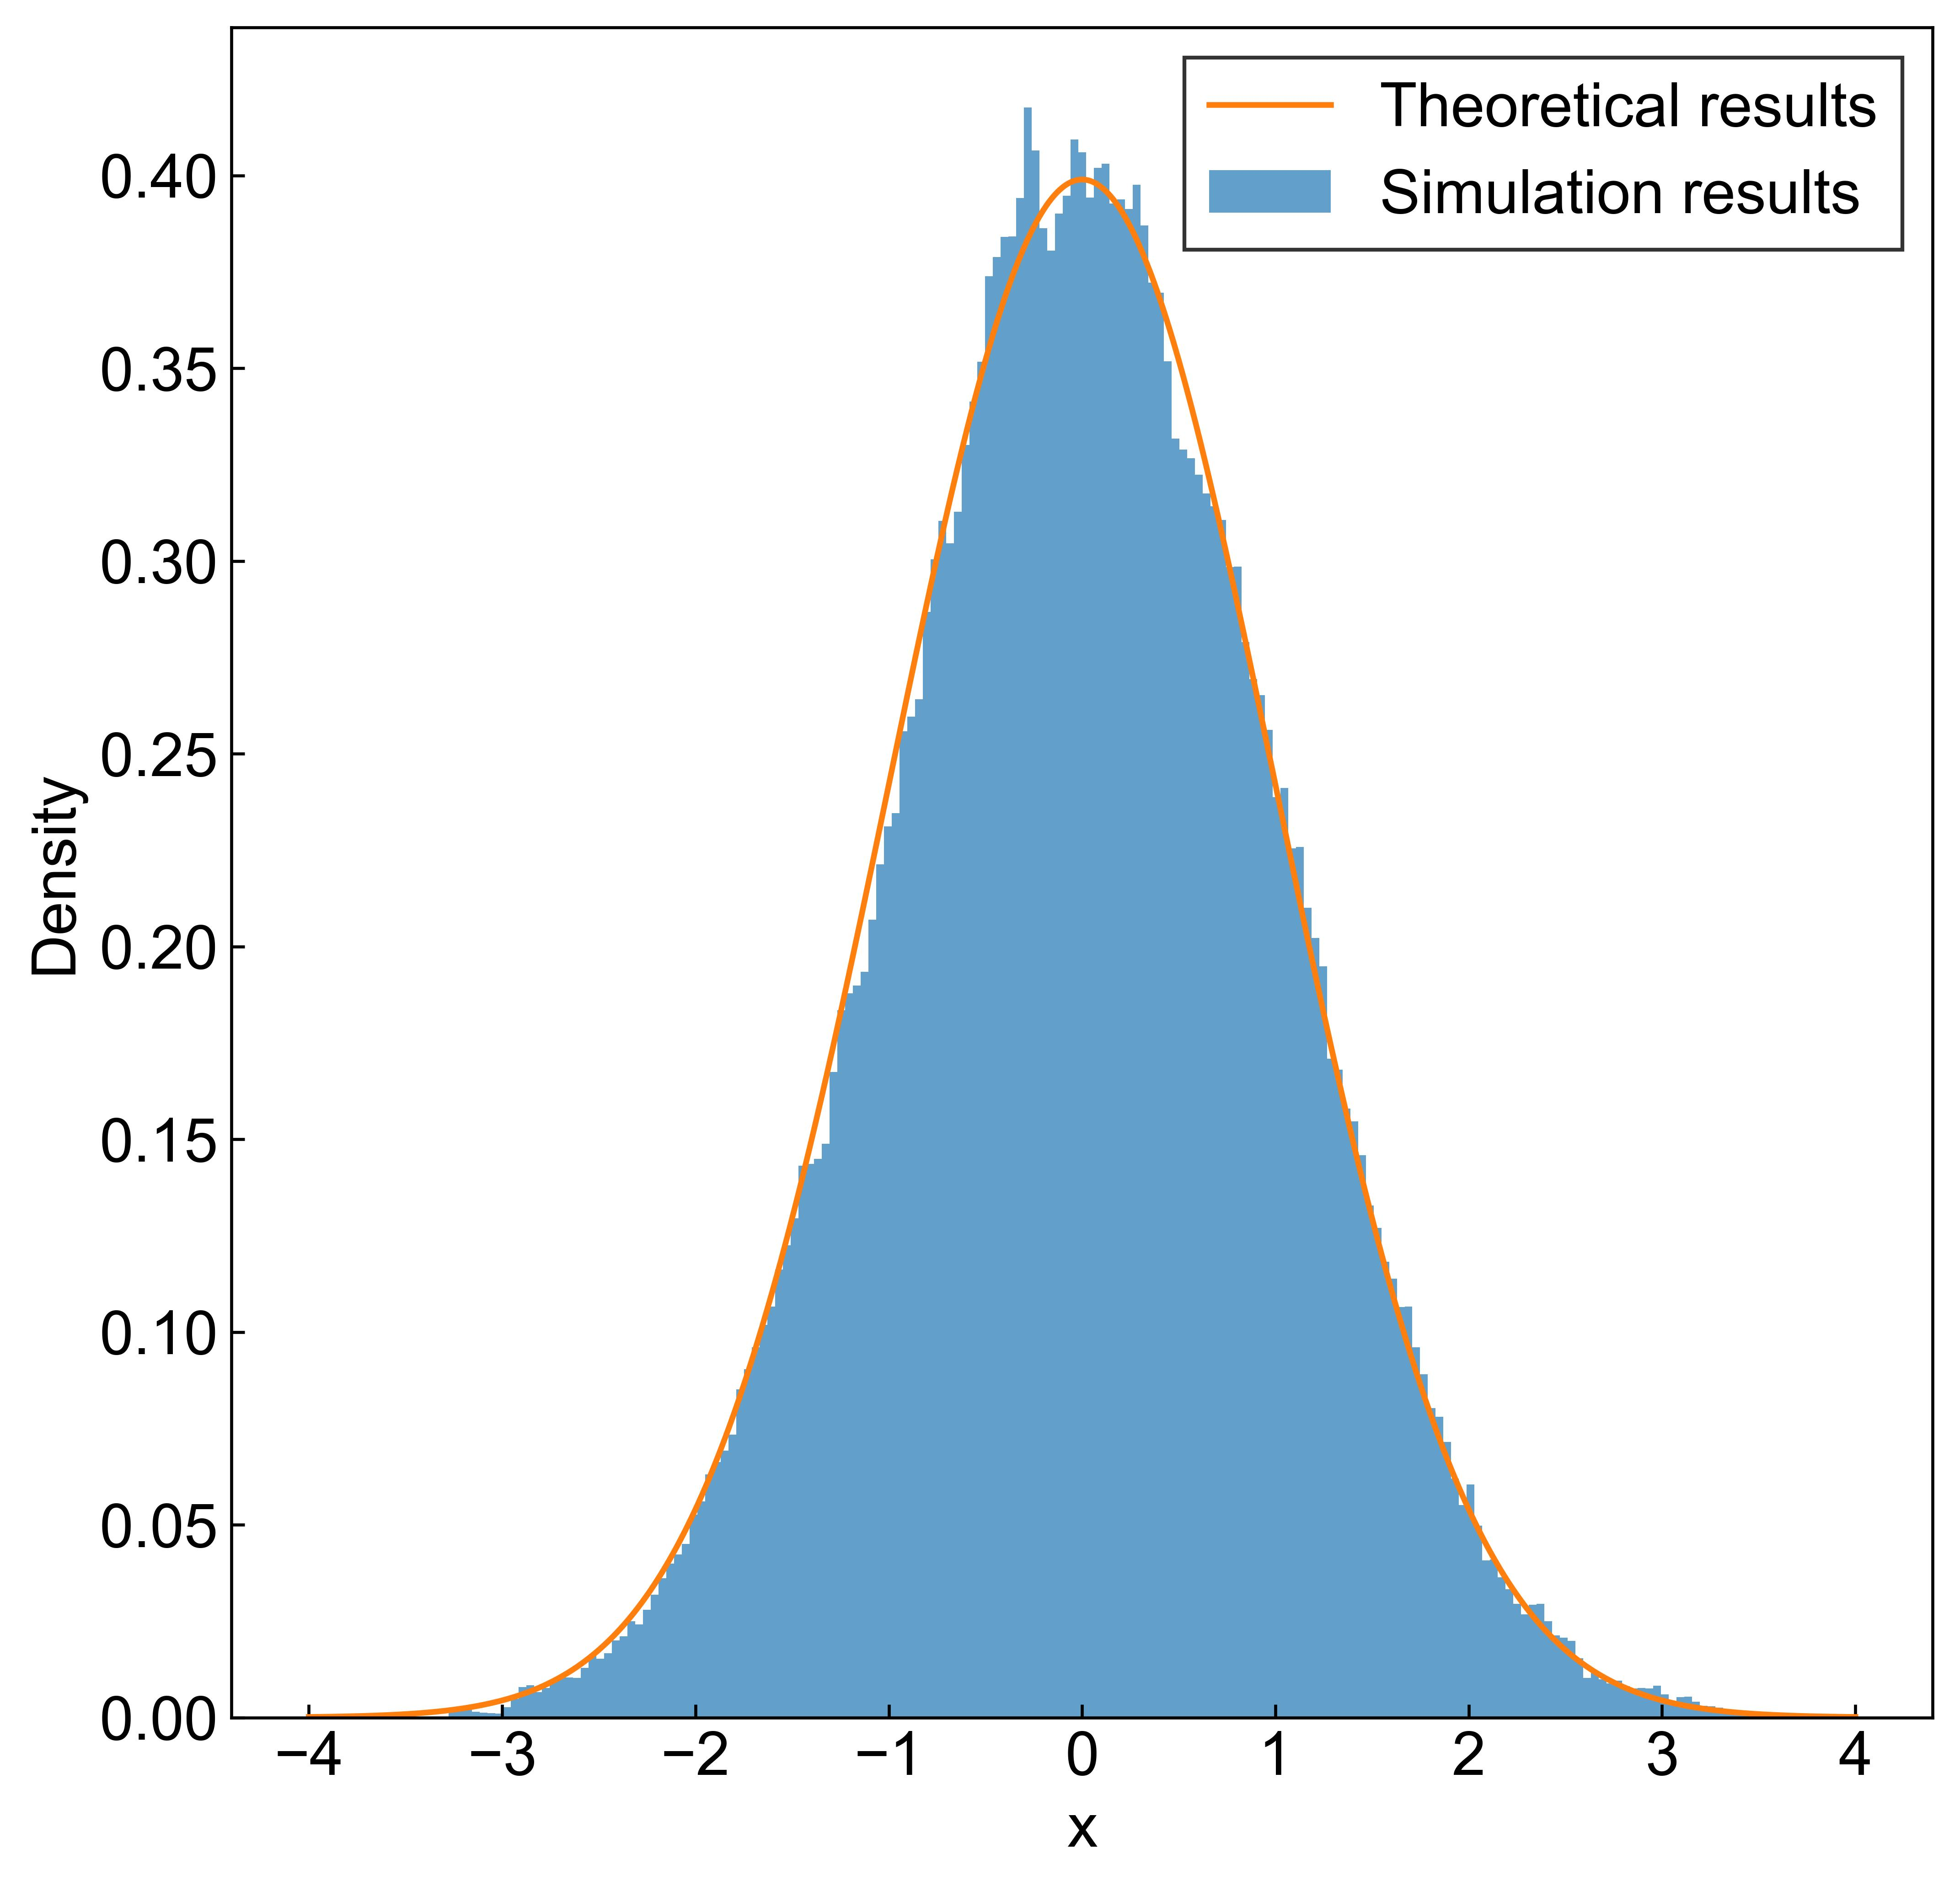
\includegraphics[width=0.48\textwidth]{NHchain-x.jpg}
    }
    \subfloat[$p$]
    {
    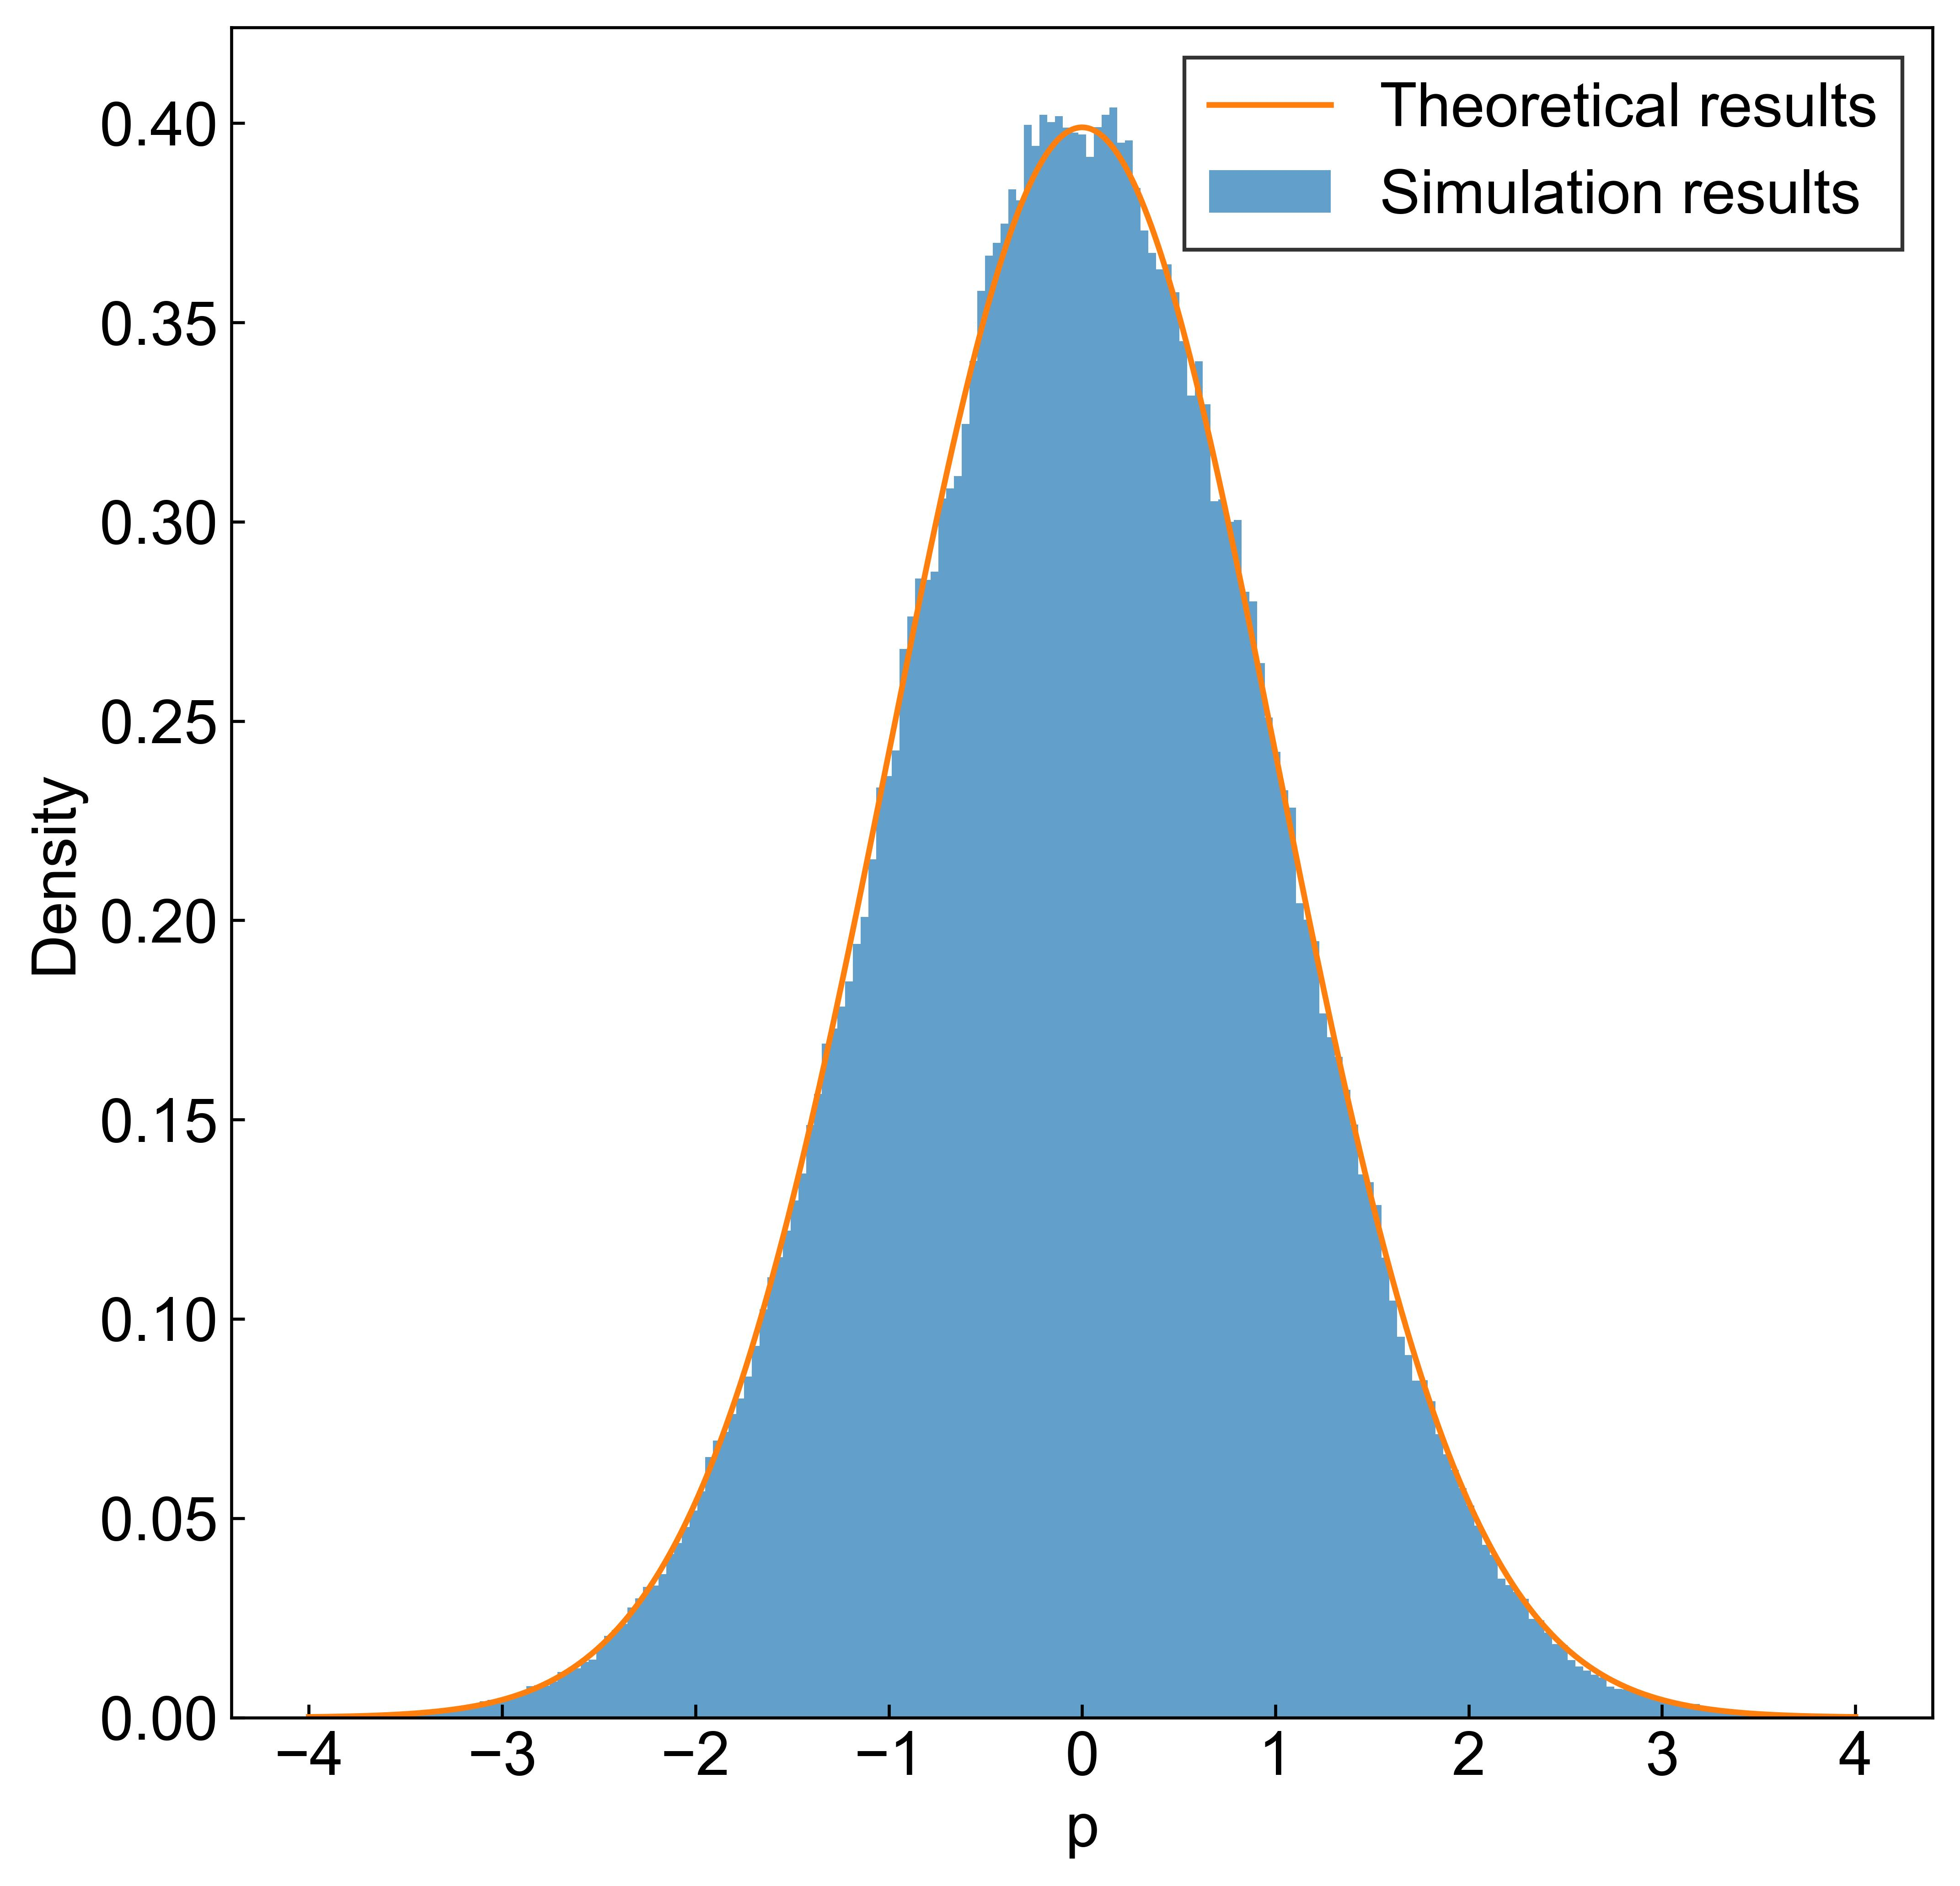
\includegraphics[width=0.48\textwidth]{NHchain-p.jpg}
    }
    \caption{The distribution of position and momentum a harmonic oscillator coupled to a Nose-Hoover chain of 6 Nose-Hoover thermostat with $Q = 0.4$. The theoretical results for canonical distribution are shown in orange curves.}
\end{figure}

\section{Coupling to a stochastic thermostat}
Consider a harmonic oscillator coupled to a stochastic thermostat with white noise:
\begin{equation}
    \begin{aligned}
        \dot{x} &= p \\
        \dot{p} &= -x-\gamma p+\eta
    \end{aligned}
\end{equation}
Here the noise term satisfies
\begin{equation}
    \begin{aligned}
        \braket{\eta(t)} &= 0 \\
        \braket{\eta(t) \eta\left(t^{\prime}\right)} &= 2 k_B T \gamma \delta\left(t-t^{\prime}\right)
    \end{aligned}
\end{equation}
The equations of motion can be solved using the following algorithm
\begin{equation}
    \begin{aligned}
        p(t^+) &= C_1 p(t) + C_2 R_1 \\
        x(t + \delta t) &= x(t) + \frac{\delta t}{m} p(t^+) + \frac{\delta t^2}{2m} F(x(t)) \\
        p(t^- + \delta t) &= p(t^+) + \frac{\delta t}{2} [F(x(t)) + F(x(t + \delta t))] \\
        p(t + \delta t) &= C_1 p(t + \delta t) + C_2 R_2
    \end{aligned}
\end{equation}
Here $C_1 = e^{-\gamma \frac{\delta t}{2}}$, $C_2 = \sqrt{\frac{1 - C_1^2}{r \delta t}}$, and $R_1$ and $R_2$ are two Gaussian random variables satisfying $\braket{R_i} = 0$ and $\braket{R_i^2} = mk_BT \gamma \delta t$, where $\gamma$ is a constant. I still take $m = \omega = 1$, $F = -x$, and $k_B T =1$. After tuning the parameters, I set $k_B T = 1$, and $\gamma = 1$. The boundary condition is set to $x_0 = 1,\ p_0 = 0$. The time step is 0.001, and the total number of steps is 10,000,000. The corresponding trajectories in the $p$-$x$ phase plane are plotted as shown in Fig. 4. The distribution of $x$ and $p$ are shown in Fig. 5, which also agrees well with the theoretical results. 

In order to better evaluate the performance of different thermostats, I plotted the distributions of position and momentum obtained from all three thermostats of my simulated distribution in Fig. 6. To fairly compare different thermostats, I set the same time step of 0.001 and the same number of total steps of 10,000,000 for all three thermostats. The density error is also shown for NH chain and stochastic thermostat, which is the absolute error of my simulations, i.e., the difference between the simulated value and the theoretical value. The results show that both NH chain and stochastic thermostat are good thermostats that can achieve almost canonical distribution of position and momentum for this harmonic oscillator system, and the stochastic thermostat does a better job considering its significantly low error in momentum distribution. However, the distribution obtained with NH thermostat greatly deviates the canonical distribution, especially for the position. In Eq. 4, Eq. 6, and Eq 10, these thermostats directly apply perturbations to the particle momentum, while the changes in position undergo a secondary effect after sensing the momentum change, thus exhibiting a certain degree of lag. This could possibly explain why the errors in the position distribution for all three thermostats are relatively greater than those in momentum.

\begin{figure}
    \centering
    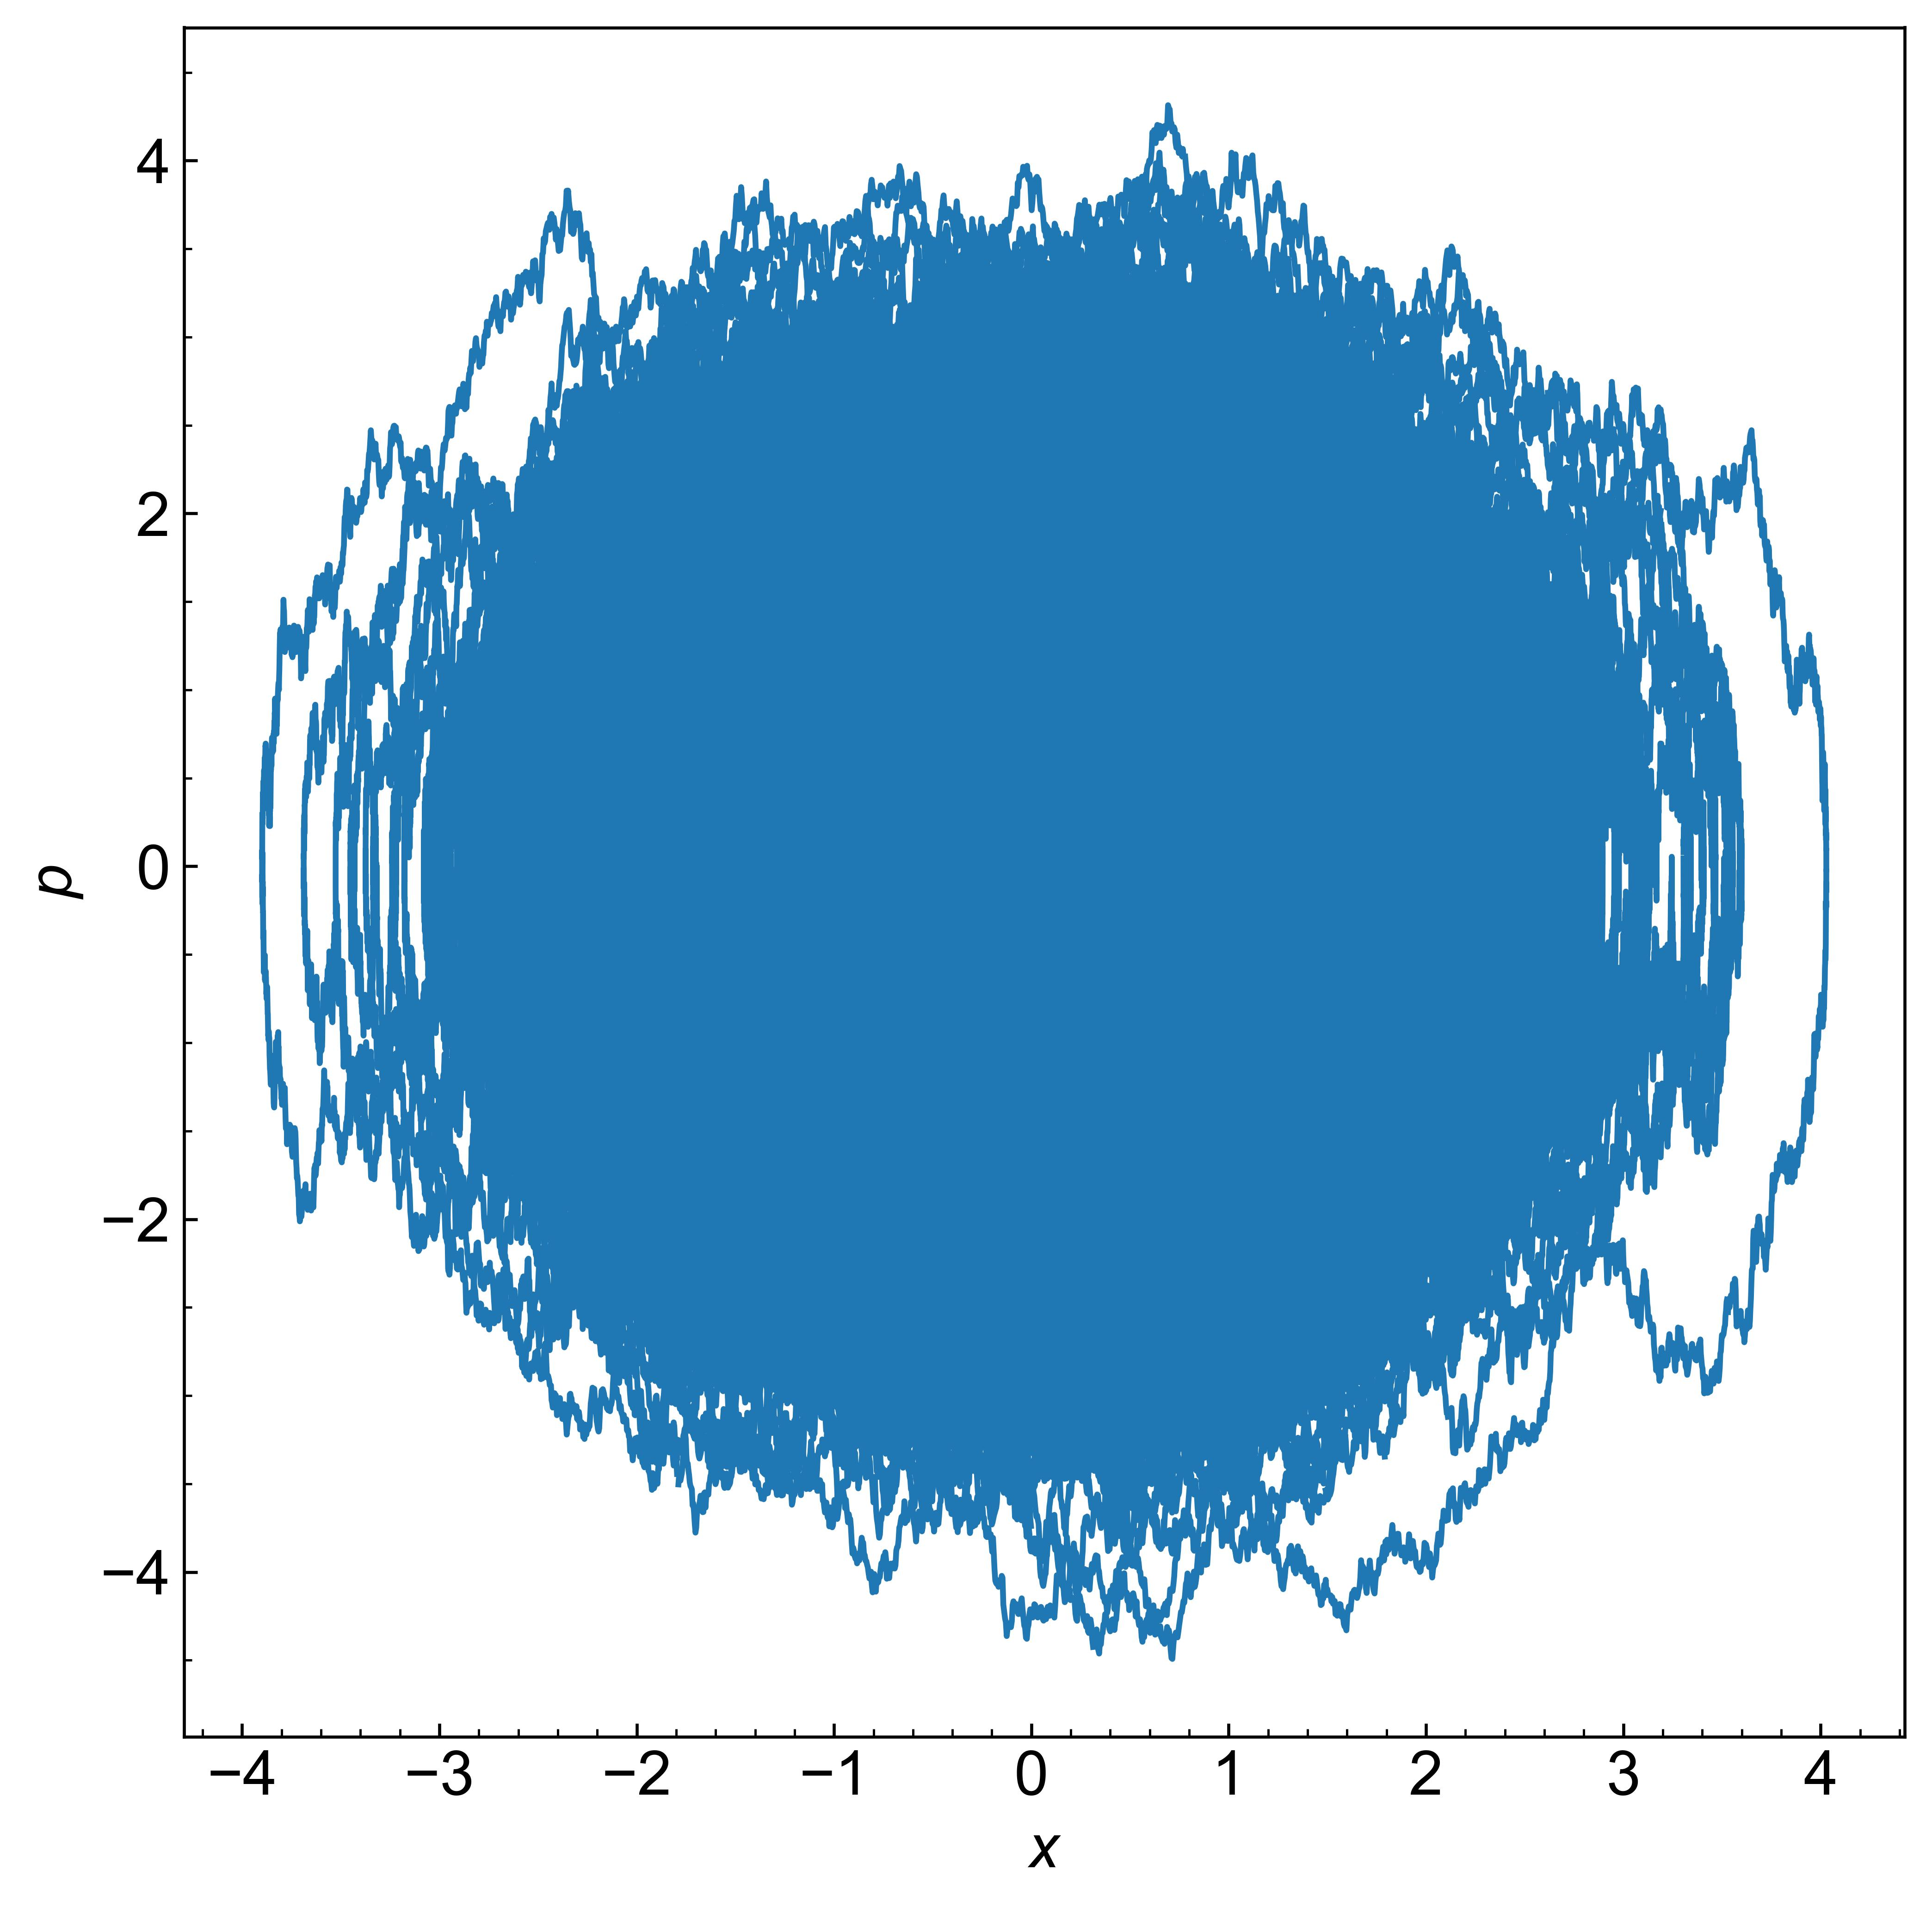
\includegraphics[width=0.65\textwidth]{stochastic.jpg}
    \caption{The trajectories in the $p$-$x$ phase plane of a harmonic oscillator coupled to a stochastic thermostat with $\gamma = 1$.}
\end{figure}
\begin{figure}
    \centering
    \subfloat[$x$]
    {
    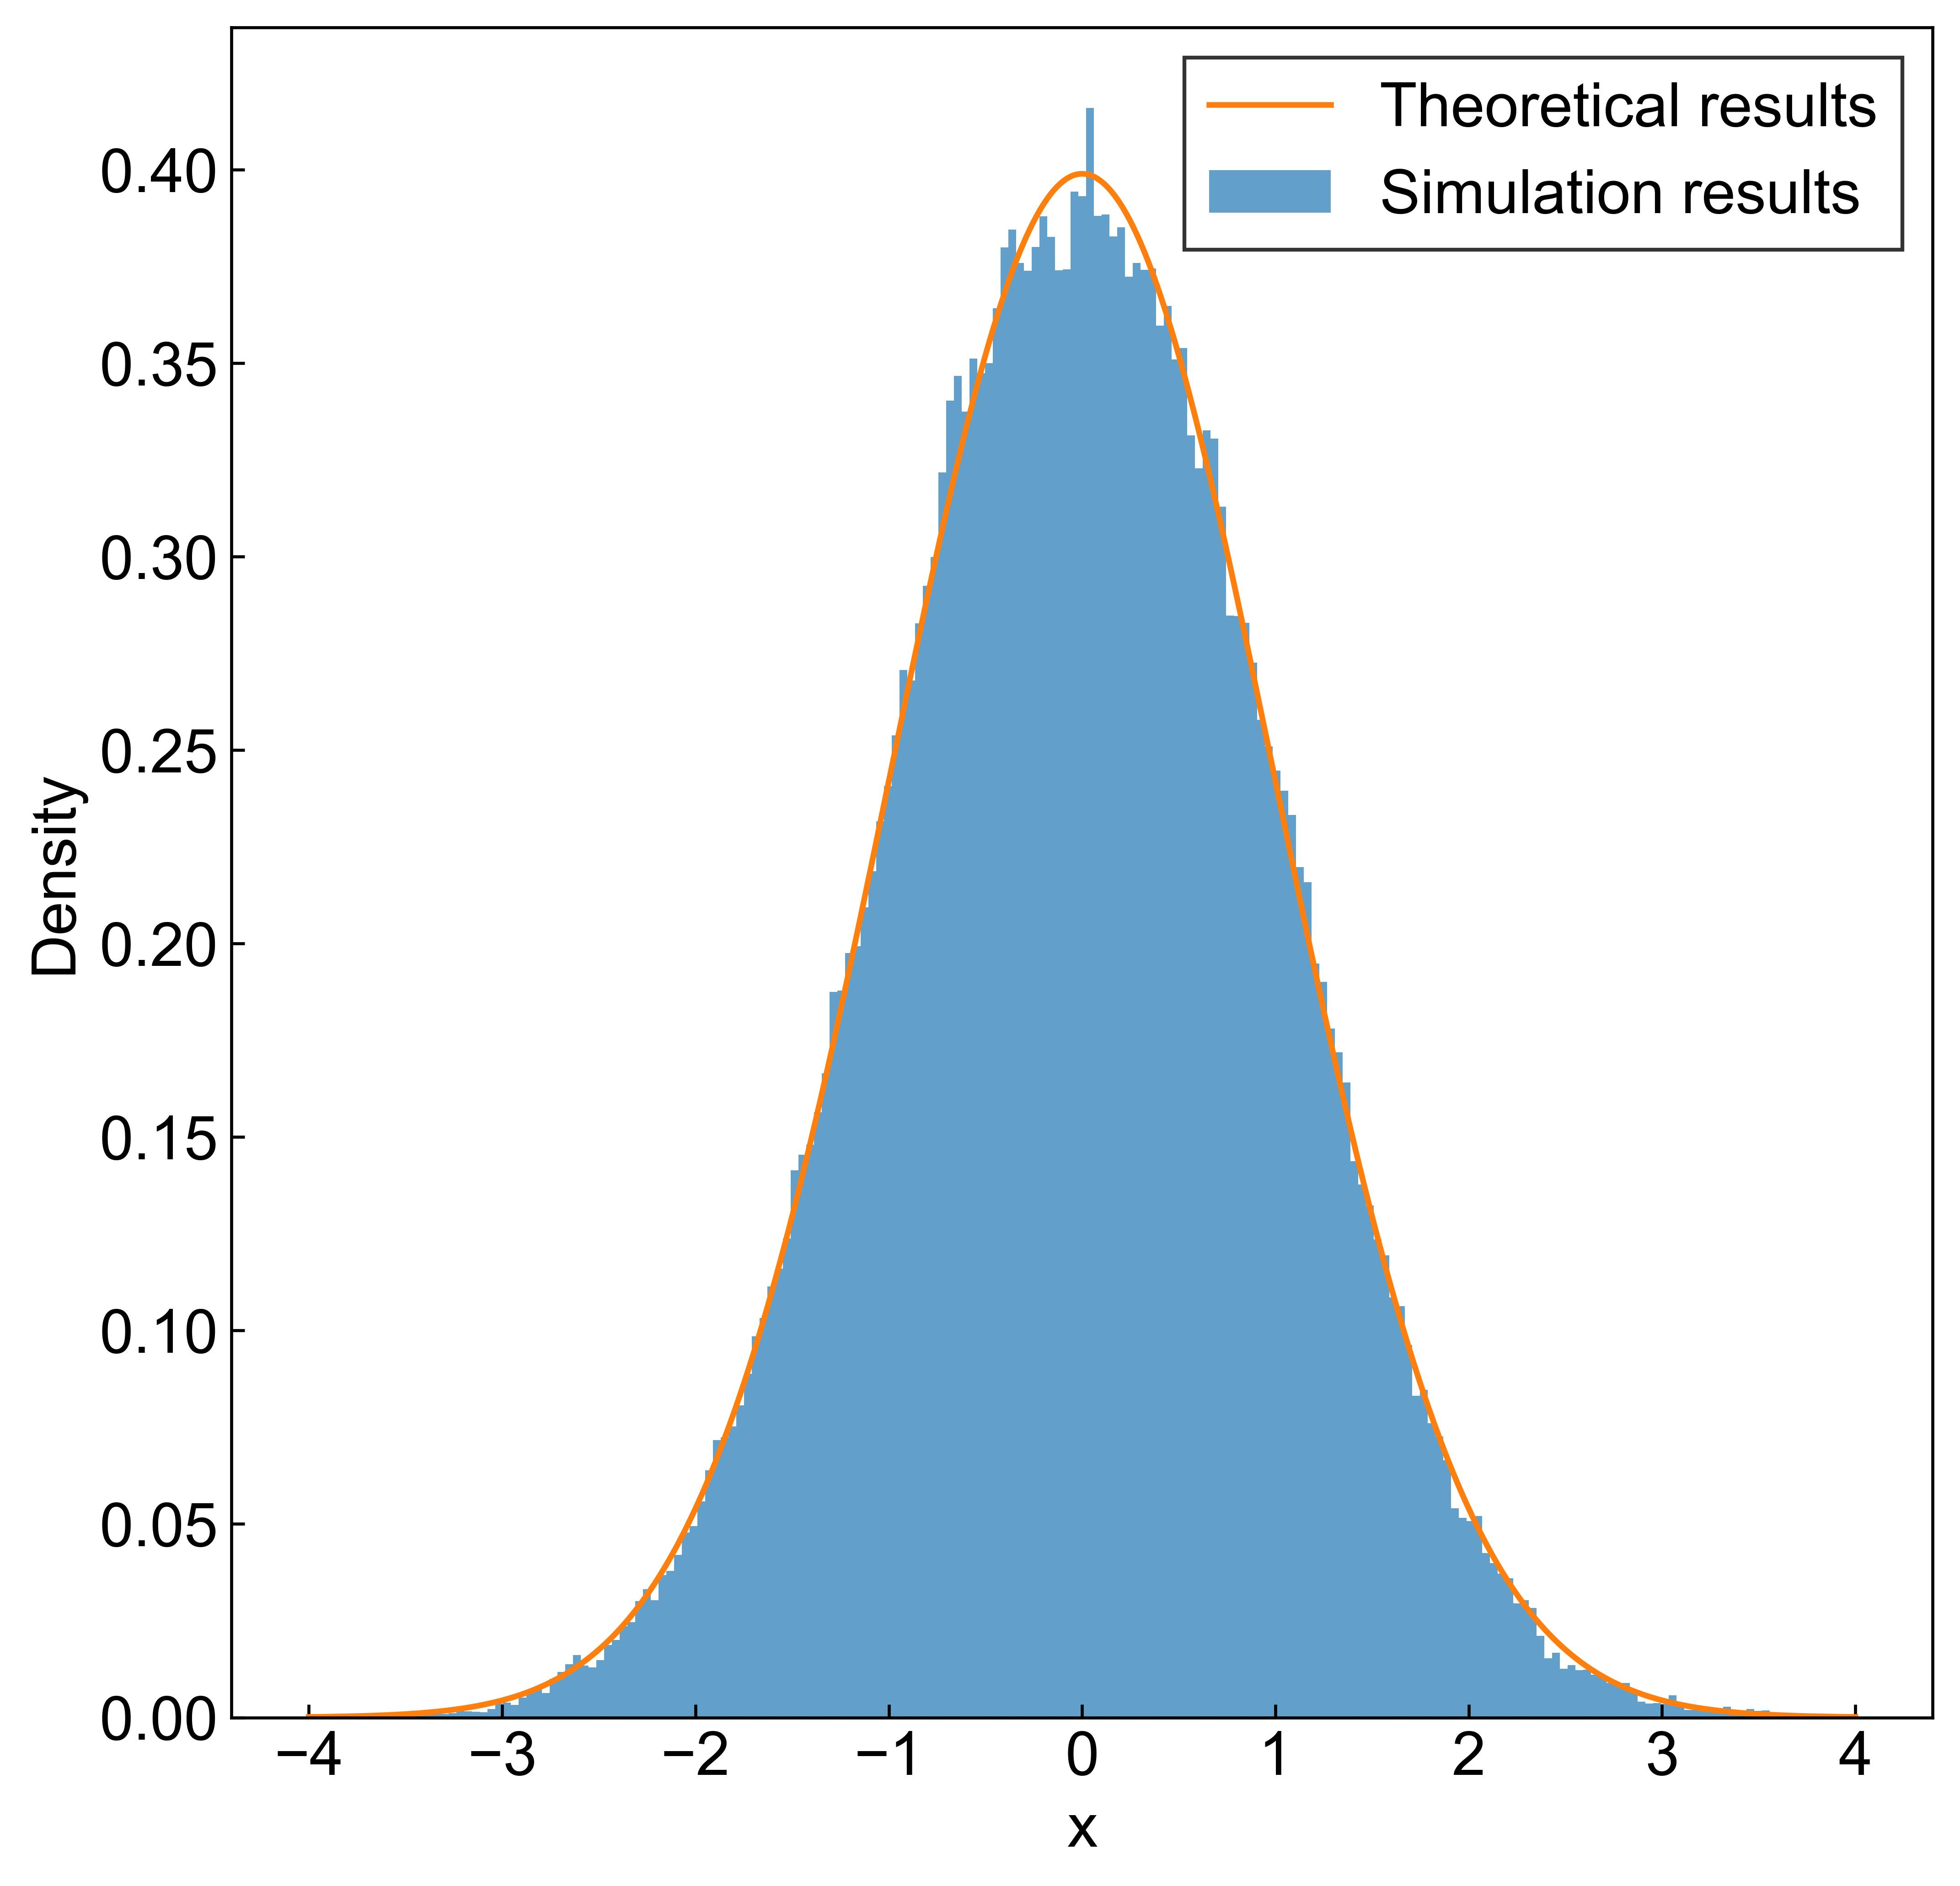
\includegraphics[width=0.48\textwidth]{stochastic-x.jpg}
    }
    \subfloat[$p$]
    {
    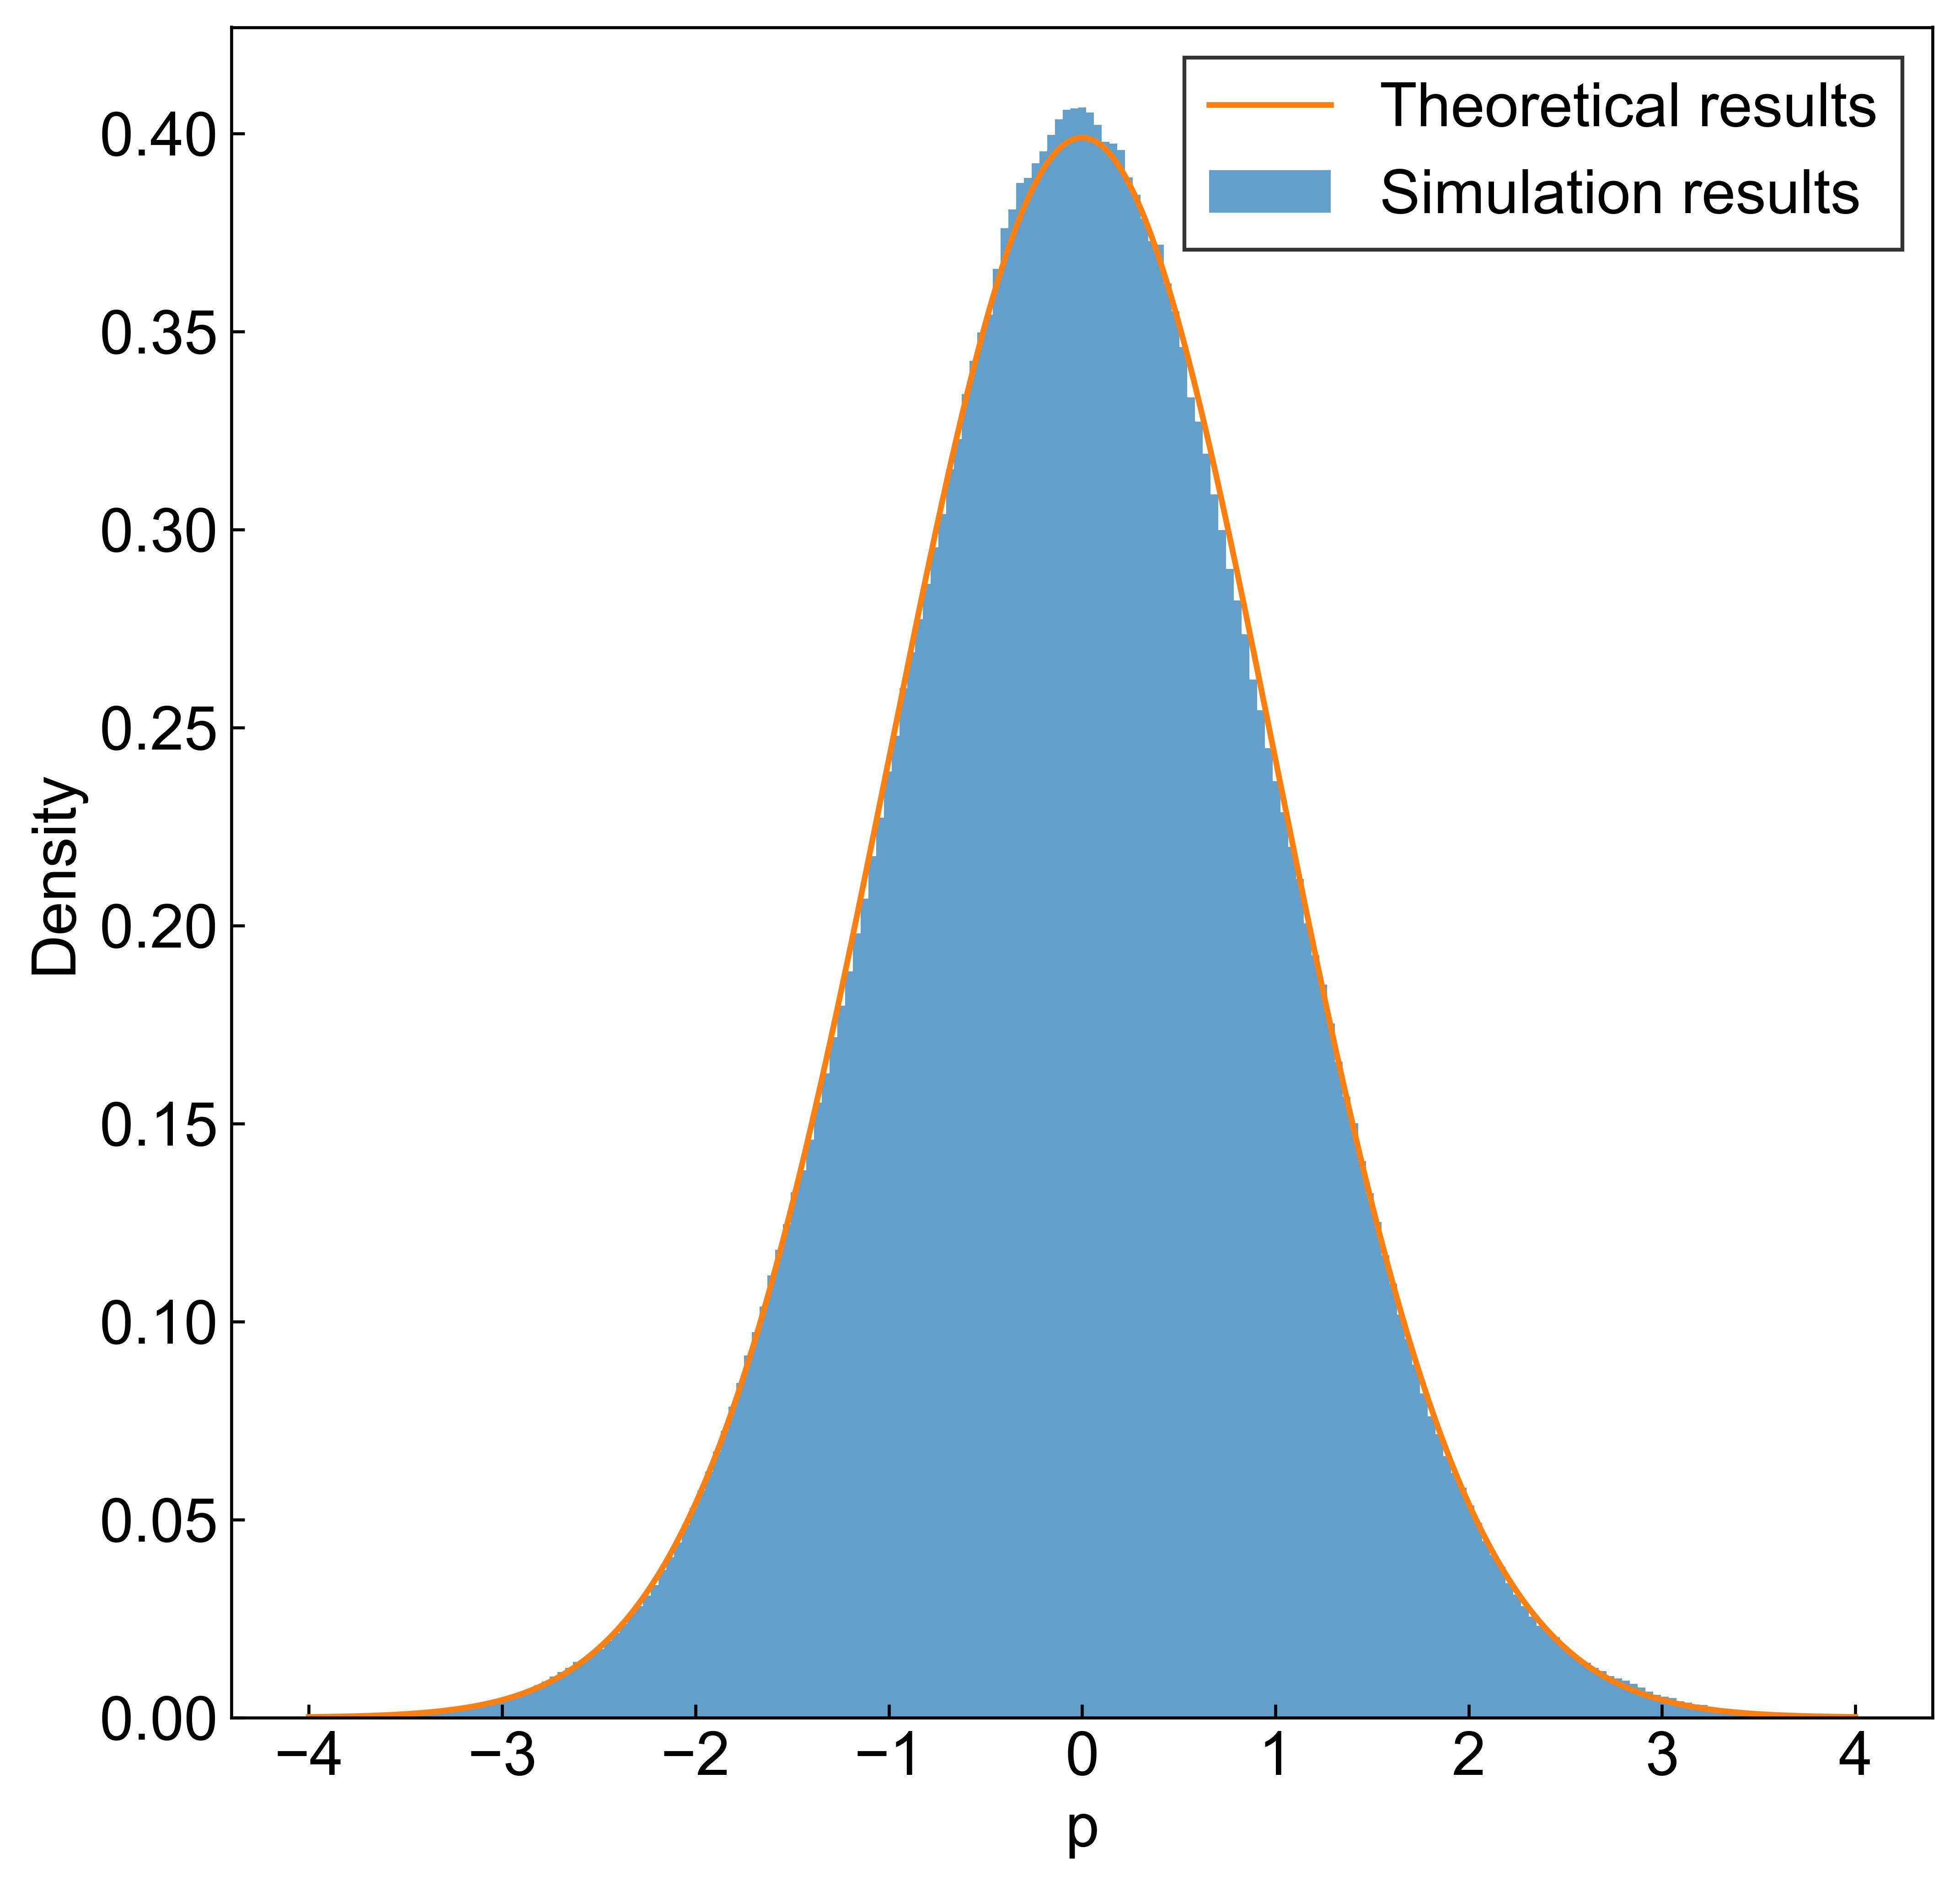
\includegraphics[width=0.48\textwidth]{stochastic-p.jpg}
    }
    \caption{The distribution of position and momentum a harmonic oscillator coupled to a stochastic thermostat with $\gamma = 1$. The theoretical results for canonical distribution are shown in orange curves.}
\end{figure}
\begin{figure}
    \centering
    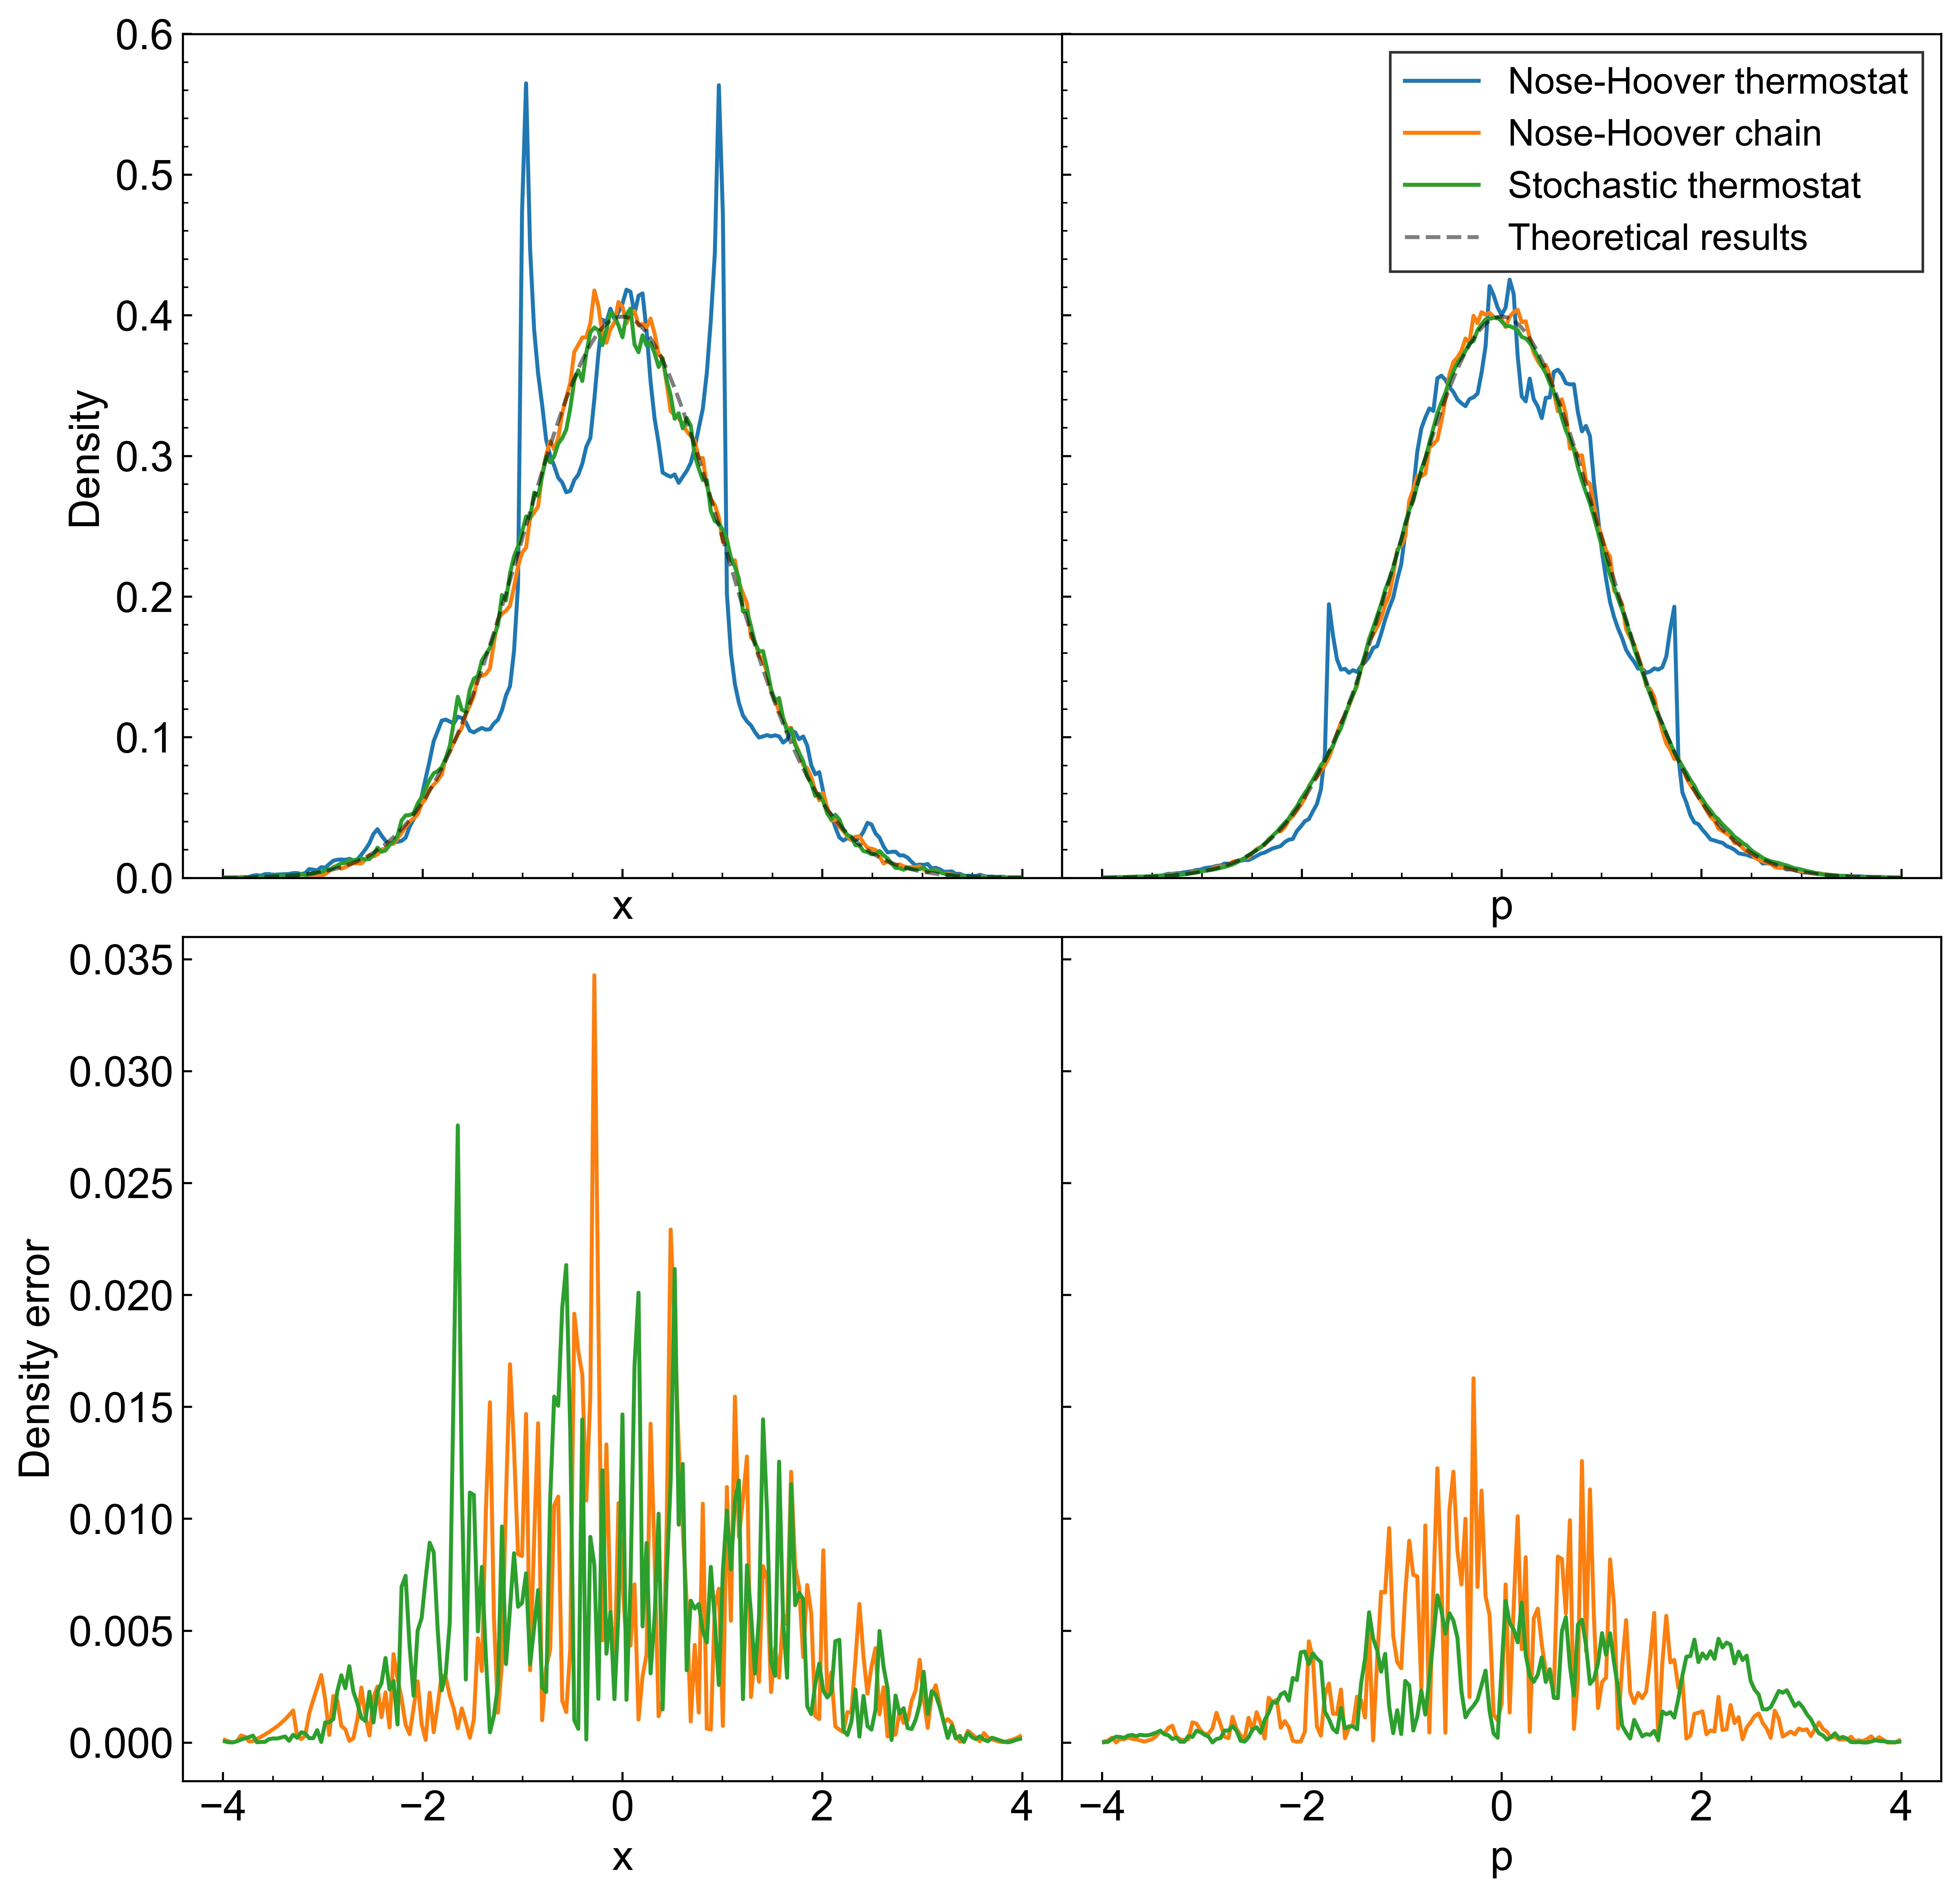
\includegraphics[width=\textwidth]{compare.jpg}
    \caption{The distribution of position and momentum a harmonic oscillator coupled to different thermostats.}
\end{figure}

\end{document}
